\chapter{听觉处理的中枢神经系统} \label{chap:chap28}

听觉对于定位和识别声音至关重要;
对于人类来说,它特别重要,因为它在理解和产生语言方面发挥着重要作用。
听觉系统有几个值得注意的特征。
它的皮层下通路比其他感觉系统的通路更长。
与视觉系统不同,声音可以从四面八方进入听觉系统,白天和黑夜,无论我们睡着还是醒着。
听觉系统不仅处理从体外发出的声音(环境声音、他人发出的声音),还处理自己产生的声音(发声和咀嚼声音)。
声音刺激在空间中的位置不是由感觉传入神经元的空间排列来传达的,而是由听觉系统根据物理线索的表示来计算的。



\section{声音向有听觉的动物传达多种类型的信息}


听觉有助于提醒动物注意看不见的危险或机会的存在,而且在许多物种中,听觉还可以作为一种交流方式。
必须从每只耳朵的声音物理特性表示中提取有关声音从何处产生及其含义的信息。
要了解动物如何处理声音,首先要考虑哪些线索可用。


大多数脊椎动物利用两只耳朵来定位水平面上的声音。
如图~\ref{fig:28_1}~所示,在该平面上不同位置的声源对两只耳朵的影响不同:声音到达较早,并且在靠近声源的耳朵处更强烈。
双耳时间和强度差异携带有关声音出现位置的信息。



% !htb
\begin{figure}[htbp]
	\centering
	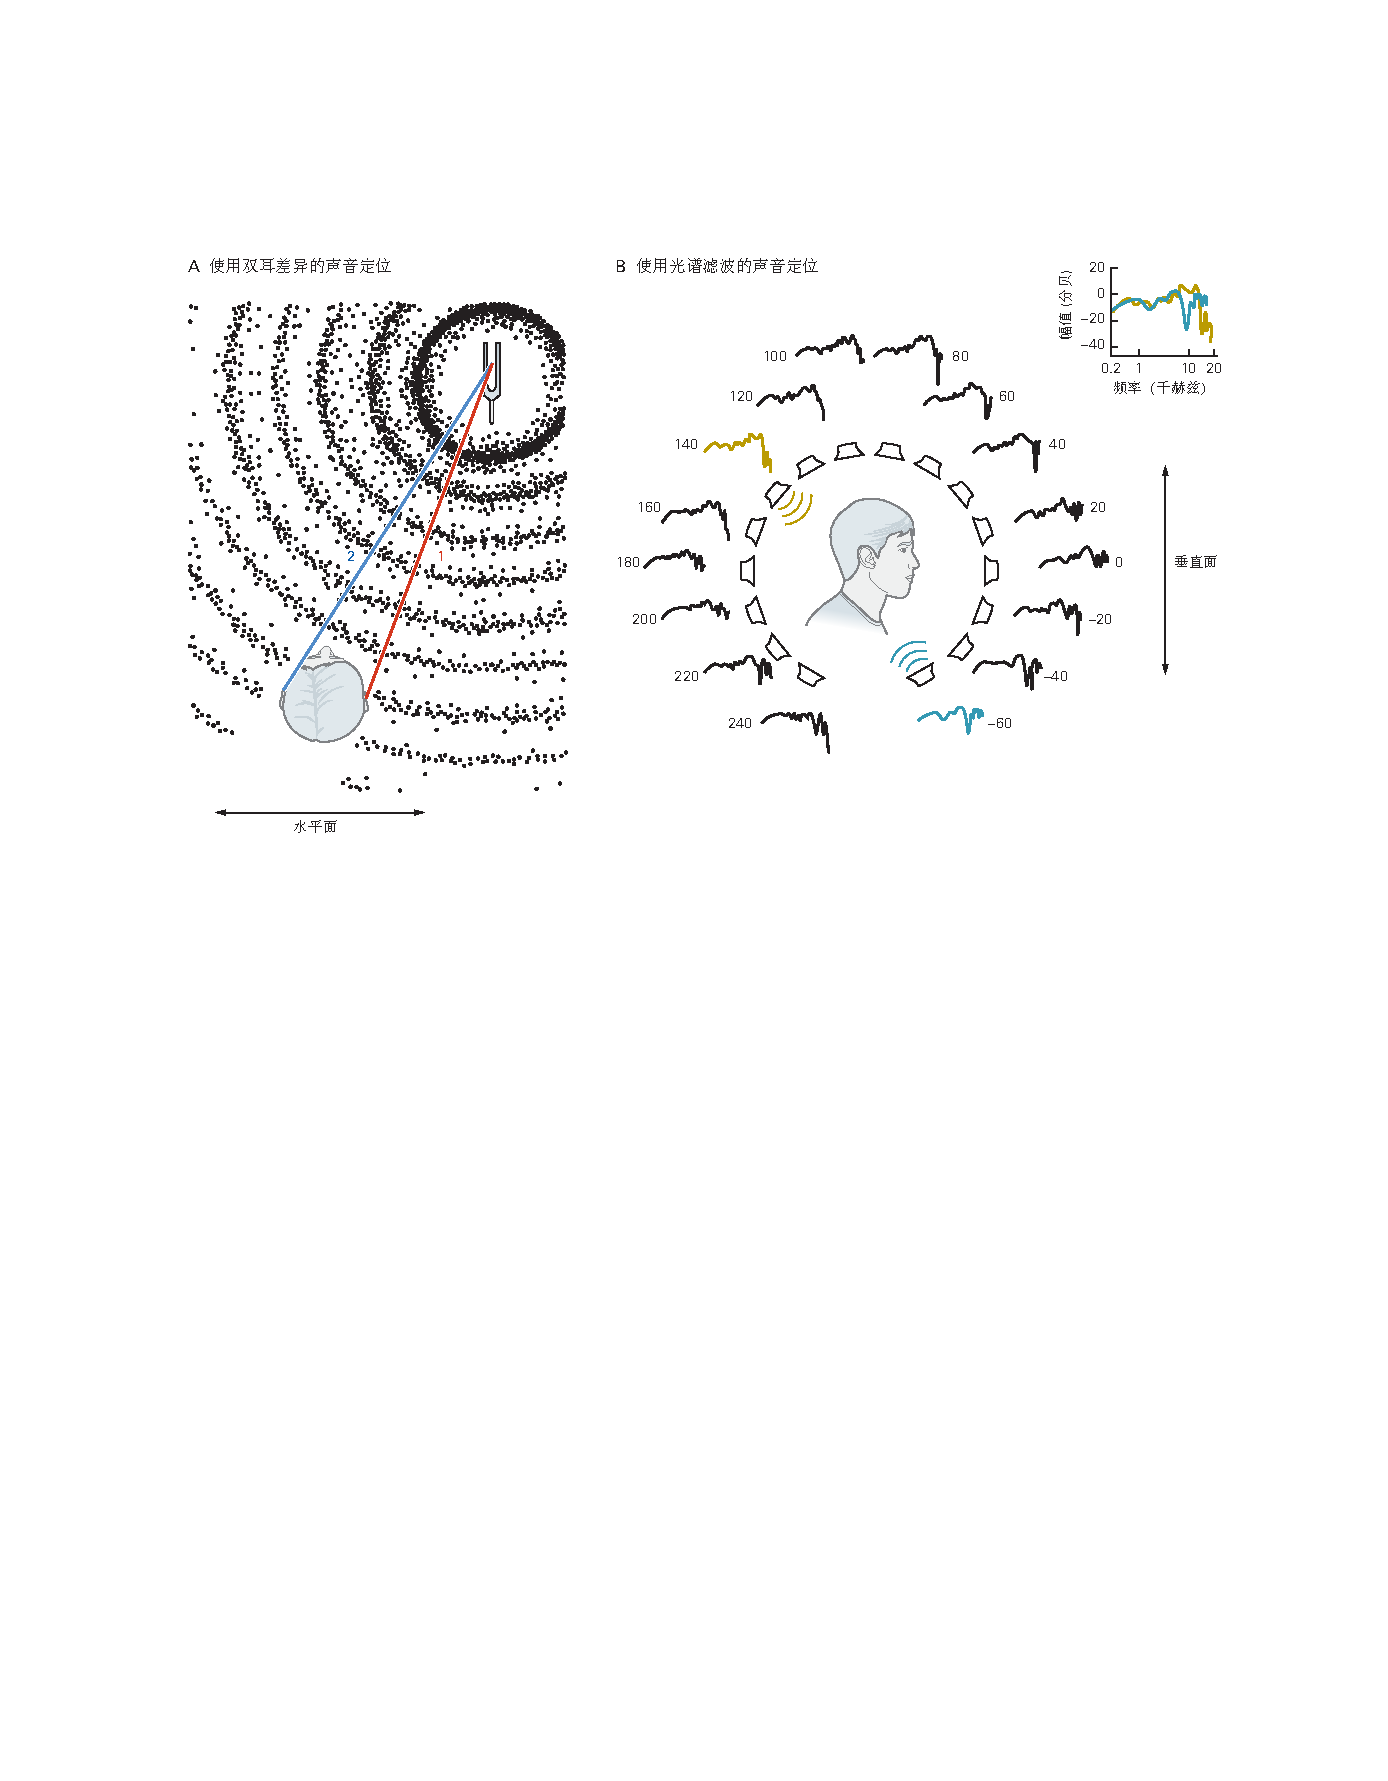
\includegraphics[width=1.0\linewidth]{chap28/fig_28_1}
	\caption{在水平面上定位声源的提示。
	A. 双耳时间和强度差异是在水平面或方位角定位声源的线索。
	在水平面上发出的声音到达两只耳朵的方式不同:声音到达的时间较早,并且越靠近声源的耳朵声音越大。
	直接从前方或后方发出的声音到达左右耳的距离相同,因此同时到达双耳。
	耳间时间和强度不随垂直平面中声源的移动而变化,因此不可能在垂直平面中定位纯正弦音调。
	在人类中,最大的耳间时间差约为 600 微秒。
	波长短的高频声音被头部偏转,在远处产生声影\cite{geisler1998sound}。
	B. 哺乳动物可以在频谱过滤的基础上在垂直和水平平面上定位宽带声音。
	当通过扬声器呈现在人类听觉范围内的所有频率上都具有相同能量的噪声(白噪声)时,耳朵、头部和肩部会抵消某些频率的能量并增强其他频率的能量。
	从扬声器发出的白噪声具有平坦的功率谱,但当噪声到达耳道底部时,其频谱不再平坦。
	在图中,耳膜处每个频率的声能相对于白噪声的声能由每个扬声器旁边的轨迹显示; 
	这些轨迹绘制了以分贝为单位的相对声音幅度与频谱频率(与头部相关的传递函数)的关系。
	右上角的小图比较了 2 种与头部相关的传递函数:一种是针对听者前方出现的低噪声(蓝色),另一种是针对来自听者脑后的噪声(棕色)。
	与头部相关的传递函数在大于 8 千赫兹的频率处具有深陷波,其频率因声音的产生位置而异。
	高频和窄带声音缺乏能量的声音很难在垂直平面上定位。
	由于光谱过滤在水平面上也会发生变化,因此它为一只耳朵失去听力的动物提供了唯一的位置提示。
	您可以通过一个简单的实验来测试这些光谱线索的显著性。
	当你的朋友在不同高度直接在你面前摇动钥匙时,闭上眼睛。
	比较在正常条件下和当你通过从后面用手指推挤耳朵的形状来扭曲它们时,你对声音定位的能力。}
	\label{fig:28_1}
\end{figure}


头部的大小决定了耳间时间延迟与声源位置的关系; 神经元回路决定带时间延迟解析的精度。
由于气压波在空气中的传播速度约为 340 米/秒,因此人类的最大耳间延迟约为 600 微秒;
在小型鸟类中,最大延迟仅为 35 微秒。
人类可以将正前方声源的位置分辨到大约 1 度以内,对应于 10 微秒的耳间时间差。
编码相对较低频率的神经元特别能很好地传达双耳时间差异。
这些神经元可以在声音的每个周期中的相同位置激活,并以这种方式将耳间时间差编码为耳间相位差。
高频声音会在两只耳朵之间产生声影或强度差异。
对于许多头部较小的哺乳动物来说,高频声音是在水平面上定位声音的主要线索。


哺乳动物可以使用频谱滤波在垂直平面和单耳中定位声音。
如图~\ref{fig:28_1}B~所示,高频声音的波长接近或小于头部、肩部和外耳的尺寸,与身体的这些部位相互作用产生相长和相消的干扰,引入宽谱峰和深而窄的谱槽,其频率随声音的位置而变化。
来自不同来源的高频声音被不同地过滤,因为在哺乳动物中,外耳的形状从后到前以及从上到下不同。
动物学会使用这些光谱线索来定位声源。
如果通过实验改变耳朵的形状,即使是成年人也可以学会使用新的光谱线索模式。
如果动物的一只耳朵失去听力,它们就会失去耳间时间和强度线索,并且必须完全依赖光谱线索来定位声音。


我们如何理解我们听到的复杂多变的声音?
大多数自然声音都包含广泛频率范围内的能量,并随时间迅速变化。
用于识别声音的信息因动物种类而异,并且取决于聆听条件和经验。
例如,人类的语言可以在噪音中、通过扭曲声音的电子设备甚至通过人工耳蜗来理解。
其稳健性的一个原因是语音包含冗余线索:发声器官产生的声音中有多个参数是共变的。
与此同时,这使得理解动物如何识别模式成为一项复杂的任务。
目前尚不清楚动物在不同条件下会使用哪些线索。


音乐是人类快乐的源泉。
乐器和人声产生的声音不仅包含与我们感知到的音高相对应的基本频率能量,还包含这个频率的多个倍数。
正是这些特性为声音赋予了独特的质感,如笛子和小提琴,让我们能够在 2 个乐器发出相同音高的情况下,区分出它们各自的声音。
音乐音高主要集中在低频范围内,在这一频率区间内,听神经纤维与声音同步发放。
在音乐中,声音的同时组合产生和弦,而连续组合产生旋律。
令人愉悦的和谐音会引起耳蜗神经纤维的规律、周期性的放电。
在不和谐的音调中,声音本身以及听神经纤维的放电都缺乏规律性;
组成不和谐音的频率成分非常接近,它们相互干扰,而不是像预期的那样周期性地相互增强。



\section{中央通路中声音的神经表征始于耳蜗核}

如图~\ref{fig:28_2}~所示,处理声学信息的神经通路从耳朵延伸到脑干,通过中脑和丘脑,到达大脑皮层。
如图~\ref{fig:26_17}~所示,声学信息从耳蜗神经节中的细胞传送到脑干中的耳蜗核。
这些信息由几种不同类型的神经元接收,其中大多数神经元按音调排列。


\begin{figure}[htbp]
	\centering
	\includegraphics[width=0.95\linewidth]{chap28/fig_28_2}
	\caption{中枢听觉通路从脑干通过中脑和丘脑延伸到听觉皮层。
		耳蜗神经(第 8 对颅神经)中的纤维终止于脑干的耳蜗核。
		这些细胞核的神经元通过几条并行通路投射到下丘。
		它们的轴突通过斜方体、中间听纹或背侧听纹退出。
		一些细胞直接终止于下丘。
		其他接触上橄榄复合体和外侧丘系细胞核中的细胞,后者又投射到下丘。
		下丘的神经元投射到上丘和丘脑的内侧膝状体核。
		丘脑神经元投射到听觉皮层。
		耳蜗核和外侧丘系的腹侧核是唯一接收单耳输入的中枢听觉神经元。}
	\label{fig:28_2}
\end{figure}


不同类型神经元的轴突采用不同的路径到达脑干和中脑,并在不同的目标处终止。
从耳蜗核到对侧下丘的一些通路是直接的;
其他涉及脑干听觉核中的 1 个或 2 个突触阶段。
从双侧下丘,声音信息以 2 种方式流动:到同侧上丘,在那里它参与调整头部和眼睛对声音的响应,以及到同侧丘脑,传递到大脑皮层的听觉区域。
从外围到更高脑区的传入听觉通路包括许多级别的传出反馈。



\subsection{耳蜗神经以并行通路将声学信息传递到音调组织的耳蜗核}

来自耳蜗神经节细胞的传入神经纤维被束缚在耳蜗或前庭耳蜗神经(第 8 颅神经)的听觉成分中,并完全终止于耳蜗核。
哺乳动物的耳蜗神经包含 2 组纤维:大量(95\%)的有髓纤维接收来自内毛细胞的输入,以及少量(5\%)的无髓纤维接收来自外毛细胞的输入。


与无髓纤维相比,有髓纤维更大、更常见,因此更容易被理解。
每种类型都检测狭窄频率范围内的能量;
因此,耳蜗神经纤维的音调阵列携带着关于声音频率内容如何随时间变化的详细信息。
无髓神经纤维既终止于耳蜗腹侧核的大神经元,也终止于耳蜗腹侧核周围的小颗粒细胞。
因为很难从这些细小的纤维中记录下来,所以它们传递给大脑的信息还没有被很好地理解。
无髓神经纤维整合来自耳蜗相对广泛区域的信息,但对声音没有响应。
有人提出,这些纤维对耳蜗损伤有响应,并会导致听觉过敏,即接触会损伤耳蜗的响亮声音后会感到疼痛。


耳蜗核的 2 个特征很重要。
首先,这些原子核按拓扑组织。
如图~\ref{fig:28_3}~所示,携带来自检测低频的耳蜗顶端信息的纤维在腹侧和背侧耳蜗核的腹侧终止; 
那些从检测高频的耳蜗基端携带信息的那些,在背侧终止。 
其次,每个耳蜗神经纤维支配耳蜗核内的几个不同区域,将具有不同投射模式的各种类型的神经元联系到更高的听觉中枢。
因此,听觉通路包括至少 4 个并行的上行通路,它们同时从耳蜗神经纤维携带的信号中提取不同的声学信息。
并联回路是脊椎动物感觉系统的一般特征。


\begin{figure}[htbp]
	\centering
	\includegraphics[width=1.0\linewidth]{chap28/fig_28_3}
	\caption{耳蜗背核和耳蜗腹核。
		A. 3 种声音频率的刺激会在 3 个位置振动示意性展开的基底膜,从而刺激不同的毛细胞群及其传入神经纤维。
		B. 耳蜗神经纤维以同位模式投射到耳蜗核。
		编码最低频率(红色)的那些耳蜗神经纤维在最靠近腹侧的地方终止,而那些编码更高频率(黄色)的耳蜗神经纤维更多终止于背侧。
		耳蜗核包括腹侧耳蜗核和背侧耳蜗核。
		每根传入纤维进入神经根并分裂成向前延伸的分支(上行分支)和向后延伸的分支(下行分支)。
		因此,腹侧耳蜗核在功能上分为前腹侧和后腹侧。}
	\label{fig:28_3}
\end{figure}



\subsection{耳蜗腹核提取有关声音的时间和频谱信息}

无层腹侧耳蜗核的主要细胞可锐化时间和光谱信息,并将其传送到听觉通路的更高中心。 
如图~\ref{fig:28_4}~所示,3 种类型的神经元混合在一起,并通过脑干形成不同的通路。


\begin{figure}[htbp]
	\centering
	\includegraphics[width=1.0\linewidth]{chap28/fig_28_4}
	\caption{耳蜗核中不同类型的细胞从耳蜗神经纤维中提取不同类型的声学信息。
		A. 新生犬耳蜗腹核中每根耳蜗神经纤维长度的末端大小和形状不同,反映了它们突触后目标的差异。 
		大端球在毛细胞上形成突触; 
		较小的按钮接触星状细胞和章鱼细胞。 
		此处显示的神经纤维采用颜色编码,如图 \ref{fig:28_3} 所示:
		黄色纤维编码最高频率,红色纤维编码最低频率\cite{y1909histologie}。
		B. 一层小鼠颗粒细胞(浅棕色)将未分层的腹侧耳蜗核(粉红色)与分层的背侧核(棕褐色和浅棕色)分开。 
		在耳蜗背核中,梭形细胞和颗粒细胞的细胞体混杂在最外层分子层和深层之间的区域。
		耳蜗神经纤维,如图~\ref{fig:28_3}~中的频率颜色编码,终止于 2 个细胞核,但在主要细胞上具有不同的汇聚模式。
		每个浓密的、星状的和梭形的细胞都接收来自少数听觉神经纤维的输入并进行尖锐调谐,而单个章鱼细胞与许多听觉神经纤维接触并进行广泛调谐。
		C. 小鼠耳蜗核主要细胞内在电学特性的差异反映在细胞中电压变化的模式上。
		当稳定去极化时,星形细胞和梭形细胞会激活重复动作电位,而多毛细胞和章鱼细胞中的重复激活会被低压激活的电导阻止。
		多毛细胞和章鱼细胞在去极化电压范围内的低输入电阻使得去极化电压变化迅速但也很小; 
		星形细胞和梭形细胞电压变化的上升和下降较慢。
		突触电位也不同。
		多毛细胞和章鱼细胞中的短暂突触电位需要更大的突触电流,但比星形细胞或梭形细胞中更持久的突触电位更忠实地编码听觉神经输入的时间。}
	\label{fig:28_4}
\end{figure}


毛细胞双侧投射到上橄榄复合体。
这条路有两部分。
一个穿过内侧上橄榄并比较声音到达两只耳朵的时间; 另一个穿过斜方体的内侧核和外侧上橄榄并比较耳间强度。
大的球状丛细胞感知低频并双侧投射到内侧上橄榄,形成检测耳间时间延迟并有助于水平面低频声音定位的回路。
小球状丛细胞和球状丛细胞感知更高的频率。
小球状丛细胞刺激同侧外侧上橄榄。
球状丛细胞通过花萼\footnote{这种突触结构特别像花萼(耳蜗核的轴突)包裹着玫瑰花(斜方体内侧核)}末梢刺激斜方体对侧内侧核中的神经元,进而抑制外侧上橄榄的主要细胞。
如图~\ref{fig:28_6}~所示,外侧上橄榄中的神经元整合了同侧兴奋和对侧抑制,以测量耳间强度并定位水平面中的高频声音源。


星状细胞广泛终止。
它们兴奋同侧耳蜗背核的神经元,斜方体腹核中的内侧橄榄蜗传出神经元,同侧外侧上橄榄附近的橄榄周核,以及外侧丘系,下丘的对侧腹核和丘脑。 
星状细胞的拓扑阵列对声音的频谱进行编码。


章鱼细胞激发对侧橄榄旁核中的靶标,并终止于外侧丘系腹侧核神经元上的大兴奋性肾盏末梢,这反过来又对下丘提供了及时的甘氨酸能抑制。
章鱼细胞检测声音的开始,使动物能够检测到短暂的间隙。
它们标记来自一个来源的光谱成分,这些成分必须一起开始。


这些通路通过腹侧耳蜗核执行的综合任务的差异反映在细胞形态上。
它们的树突形状反映了它们从耳蜗神经纤维收集信息的方式。
高度调谐的毛细胞和星状细胞的树突从相对较少的耳蜗神经纤维接收输入,而相比之下,广泛调谐的章鱼细胞的树突垂直于耳蜗神经纤维的路径,准备接收来自许多耳蜗神经纤维的输入。
毛细胞的许多输入来自包裹毛细胞体的异常大的终端,满足它们对大突触电流的需要。
章鱼细胞对大突触电流的需求是通过对来自大量小终端的输入求和来满足的。


神经元的生物物理学特性决定了突触电流如何转化为电压变化,以及突触输入被整合的时间长短。
腹侧耳蜗核中的章鱼和毛细胞能够以异常快速和精确定时的突触电位做出响应。
如图~\ref{fig:28_4}C~所示,这些神经元具有显著的低电压激活~\ce{K+}电导,可提供低输入电阻和快速响应并防止重复激活。
在这些渗漏细胞中触发动作电位所需的大突触电流通过许多突触处的快速门控、高电导、\textit{$\alpha$-氨基-3-羟基-5-甲基-4-异恶唑丙酸}谷氨酸受体传递。
相比之下,即使相对较小的去极化电流也会产生较大的持续电压变化的星状细胞会响应突触电流而产生较慢的\textit{兴奋性突触后电位},而\textit{N-甲基-D-天冬氨酸}型谷氨酸受体会增强这些响应。



\subsection{耳蜗背核将声学与体感信息相结合,利用频谱线索定位声音}

在脊椎动物中,只有哺乳动物具有背侧耳蜗核。
如图~\ref{fig:28_4}A、B~所示,耳蜗背核接收来自投射到不同层的 2 个神经元系统的输入。
它的主要细胞梭形细胞整合了这 2 个输入系统,并将结果直接传送到对侧下丘。


最外层的分子层是平行纤维系统的末端,颗粒细胞的无髓鞘轴突散布在耳蜗核内和周围。
该系统将体感、前庭和听觉信息从大脑的广泛区域传输到分子层。


深层接收声音信息。
耳蜗神经纤维和腹侧耳蜗核的星状细胞均终止于深层。
声学输入按音调分布在与平行纤维成直角的等频层中。


梭形细胞是耳蜗背核的主要细胞,整合了 2 个输入系统。
分子层中的平行纤维通过分子层顶端树突上的刺激发梭形细胞。
平行纤维也终止于车轮细胞的树突棘,中间神经元与小脑浦肯野细胞非常相似,后者反过来抑制梭状细胞。
腹侧耳蜗核中的耳蜗神经纤维和星状细胞通过深层光滑基底树突上的突触激发梭状细胞和抑制性中间神经元。


最近的实验表明,耳蜗背核的回路可以区分不可预测和可预测的声音。
例如,动物自己的咀嚼或舔舐声音是可以预测的,并通过这些回路消除。
当动物移动头部、耳朵或肩膀时出现的光谱线索变化,改变了声音入射到耳朵的角度,这是不可预测的,尤其是当外部声源移动时。
关于头部和耳朵位置的体感和前庭信息,以及来自更高层次神经系统的关于动物自身运动的下行信息,通过分子层调制到达深层的声学信息。



\section{哺乳动物的上橄榄复合体包含用于检测耳间时间和强度差异的独立回路}

在许多脊椎动物中,包括哺乳动物和鸟类,上橄榄复合体中的神经元比较双侧耳蜗核中细胞的活动以定位声源。
单独的回路检测耳间时间和强度差异并投射到下丘。



\subsection{内侧上橄榄生成耳间时差图}

到达耳朵的时间差异不会在耳蜗中表现出来。
相反,它们首先出现在内侧上橄榄中,通过比较两耳声音响应中动作电位的时间来创建耳间相位图。
如图~\ref{fig:28_5}A~所示,声音在到达远耳之前先到达近耳,双耳时间差与声源在水平面上的位置直接相关。


\begin{figure}[htbp]
	\centering
	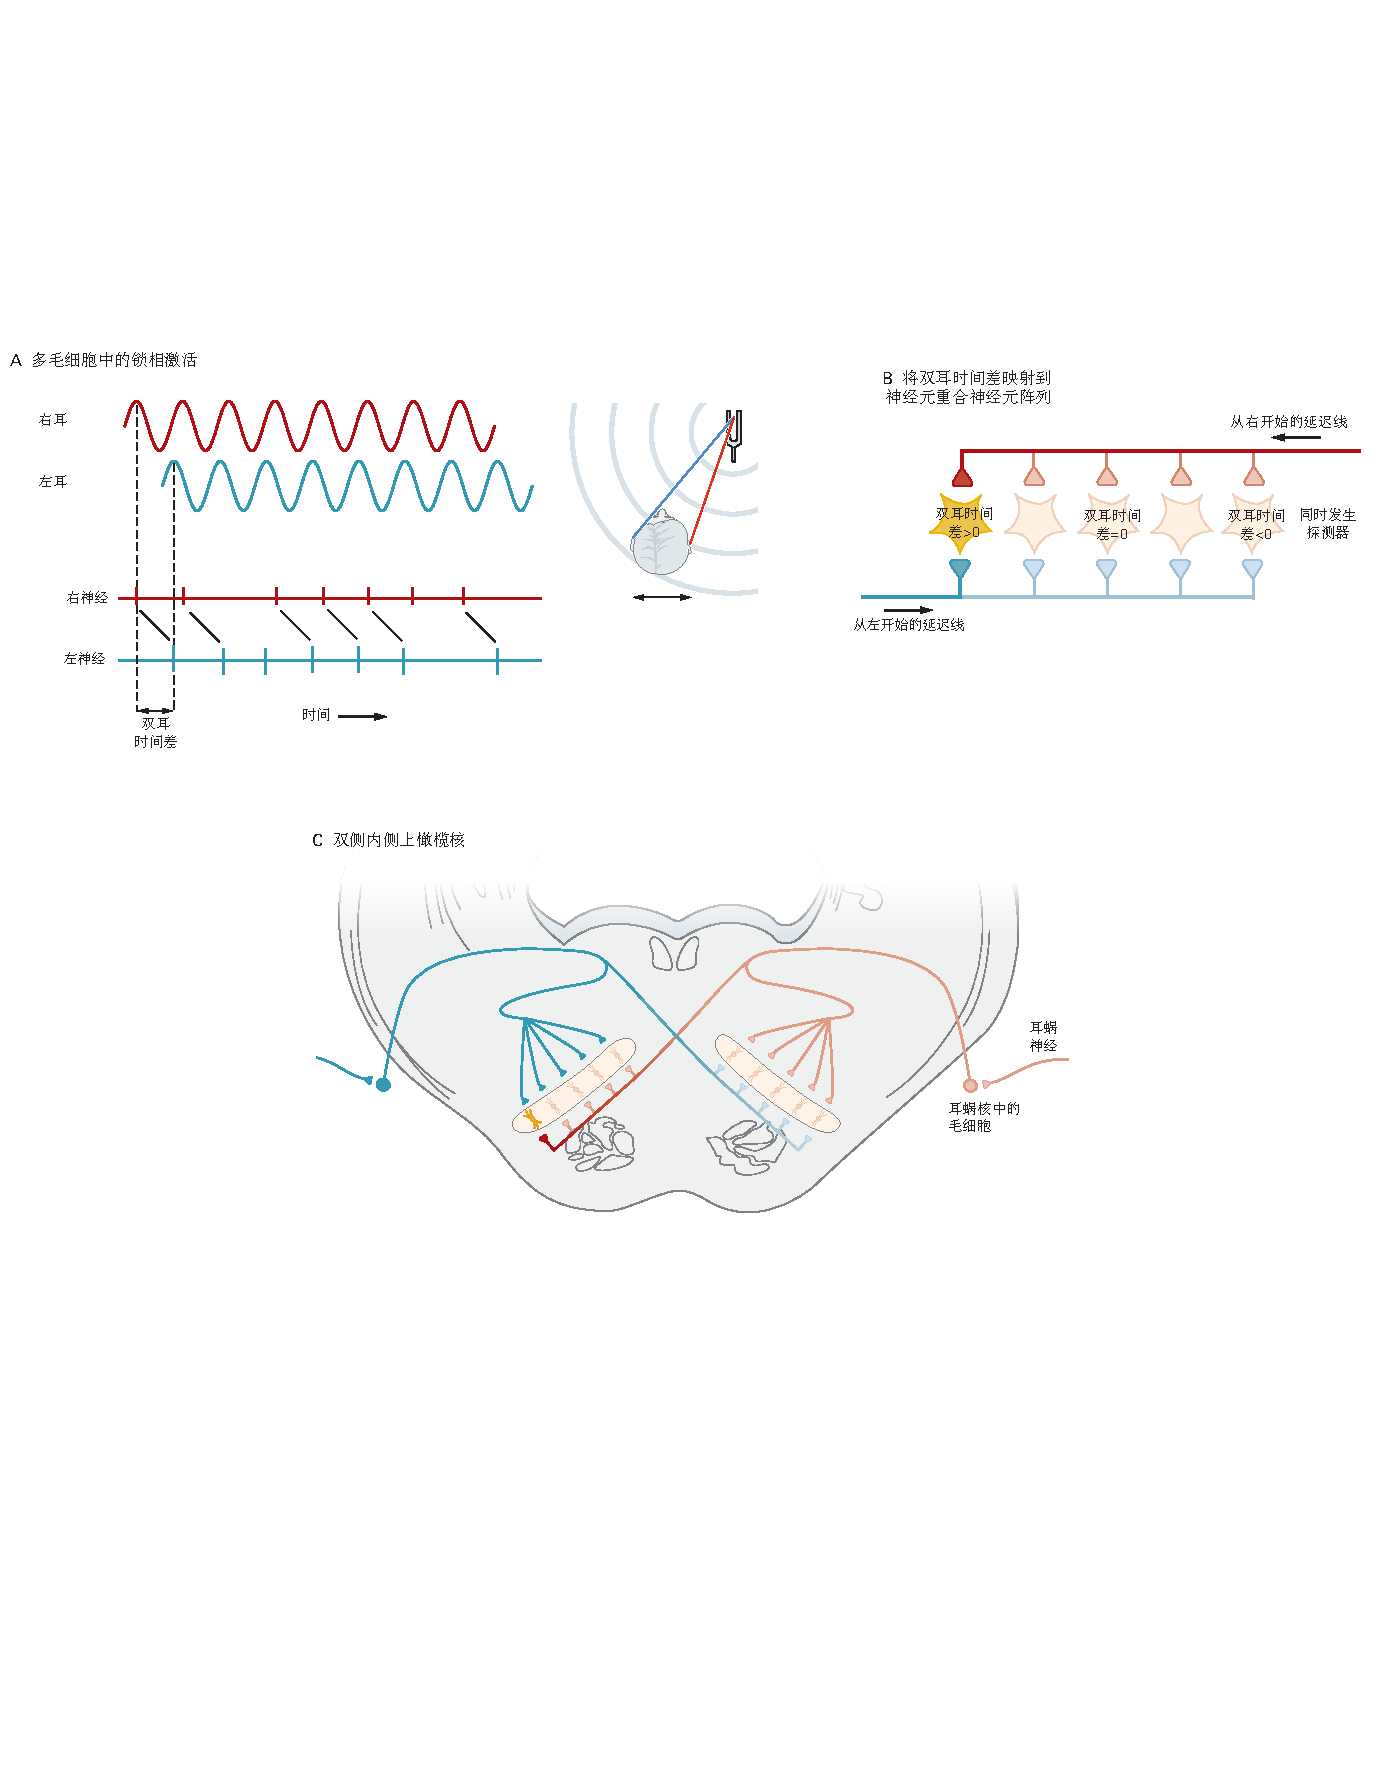
\includegraphics[width=0.9\linewidth]{chap28/fig_28_5}
	\caption{声音到达时的双耳差异有助于将声音定位在水平面上。
		A. 当从右侧发出纯音等声音时,右耳比左耳更早察觉到声音。 
		到达两只耳朵的时间差就是\textit{双耳时间差}。 
		耳蜗神经纤维及其浓密的细胞目标随着压力的变化而同步激活。
		尽管单个毛细胞可能无法在某些周期内激活,但一组细胞将编码低频声音的时间及其每个周期的频率。 
		比较两侧多毛细胞中动作电位的开始,揭示了\textit{双耳时间差}(斜黑线)。 
		B. 耳间时间差可以通过一组神经元来测量,其来自两只耳朵的输入是延迟线\cite{jeffress1948place}。
		动作电位先传播到最近的末梢,然后再到达最远的末梢;
		因此,在右边的延迟线中,终端将从右到左顺序产生突触电位,而在左边的延迟线中,终端将从左到右顺序产生突触电位。
		假设这样的突触后神经元是\textit{同时发生探测器},仅当它们同时从左右接收到\textit{兴奋性突触后电位}时才会激活。
		在中线出现的声音同时到达右耳和左耳,没有耳间时间差异(\textit{双耳时间差} = 0)。
		阵列中间的神经元从两侧接收来自同样长的轴突的输入,因此将同时接收来自两侧的\textit{兴奋性突触后电位}。
		当声音来自右侧时,来自右耳的信号比来自左耳的信号更早到达中枢神经系统(\textit{双耳时间差}大于 0)。
		来自右侧的声音在(黄色)神经元中产生同步\textit{兴奋性突触后电位},因为来自右侧(红色)的声音较早到达,由相对于来自左侧(蓝色)的声音较长的传导延迟来补偿。
		同样,当声音从左侧发出时,\textit{双耳时间差} 小于 0 并且来自左侧的传导延迟(蓝色)补偿了左侧的早期到达。
		这样的神经元回路会在重合检测器中生成双耳时间差异图;
		当声音从右到左移动时,它们会从左到右依次激活重合检测器。
		这种延迟线的排列已在谷仓猫头鹰的层状核中发现,它是哺乳动物内侧上橄榄核的同系物。
		C. 哺乳动物仅在声源对侧的细胞核中使用延迟线来形成耳间时间差异图。
		内侧上橄榄核的簇状神经元形成一张薄片,在其侧面与来自同侧耳蜗核的毛细胞接触,在内侧与来自对侧耳蜗核的毛细胞接触(虽然它在这里示意性地描绘在脑干的冠状部分,但耳间差异的编码在一张神经元中,该神经元也具有延喙尾维度)。
		在同侧,毛细胞轴突的分支是相等的长度,从而同时在内侧上橄榄的目标中启动突触电流。
		在对侧,分支首先依次将突触电流传递到最靠近中线的区域,然后逐渐传递到更侧向的区域。
		仅当声音从对侧半空间发出时,内侧上橄榄的神经元才会检测到来自两只耳朵的同步兴奋。
		当声音从右侧发出时,它们提前到达右耳会被逐渐延长的传导延迟所补偿,以激活越来越多朝向左内侧上橄榄外侧端的神经元(黄色细胞被来自远处的声音激活) 对,如 B 部分)。
		当声音从前方发出且没有双耳时间差时,内侧上橄榄前端的神经元会从两侧同步激活。
		每个内侧上橄榄形成一张映射,显示对侧半场的声音出现位置\cite{yin2002neural}。}
	\label{fig:28_5}
\end{figure}


调谐到四千赫兹以下频率的耳蜗神经纤维及其毛细胞目标通过与压力波同相激活来编码声音。
此属性称为\textit{锁相}。
尽管单个神经元可能无法在某些周期内激活,但某些神经元组会在每个周期内激活。
在这样做的过程中,这些神经元携带有关声音每个周期的输入时间信息。 
从一侧到达的声音会引起锁相激活,这种激活在近耳处始终比在远耳处更早,从而导致一致的耳间相位差(图 ~\ref{fig:28_5}A)。


如图~\ref{fig:28_5}B~所示,来自两只耳朵的重合输入的检测器阵列,通过由具有系统不同长度的轴突组成的\textit{延迟线}传输,可以形成耳间时间差异图,从而形成声源位置图\cite{jeffress1948place}。
在这样的回路中,传导延迟补偿了较早到达近耳的情况。
随着声音从中线移动到侧面,双耳时间延迟系统地增加,导致向神经元阵列的边缘进一步同步激活。


此类神经元图谱已在仓鸮的内侧上橄榄核同系物中发现。
哺乳动物和鸡使用这种输入排列的变体。
内侧上橄榄的主要神经元在中线的每一侧形成一个或几个细胞厚度的薄片。 
如图~\ref{fig:28_5}C~所示,每个神经元有两簇树突,一个延伸到薄片的侧面,另一个延伸到薄片的内侧。
侧面的树突与来自同侧耳蜗核的大球状丛细胞轴突接触,而内侧的树突与来自对侧耳蜗核的匹配最佳频率的大球状丛细胞接触。
如图~\ref{fig:28_5}C~所示,正如\textit{杰夫里斯}所建议的那样,毛细胞的轴突终止于具有延迟线的对侧内侧上橄榄,但终止于同侧内侧上橄榄的分支长度相等。


传导延迟使得每个内侧上橄榄只有在声音来自对侧一半空间时才会从两只耳朵接收一致的兴奋性输入。
当声源从中线移动到头部对侧的最外侧点时,声音较早到达对侧耳朵需要通过连续更长的延迟线来补偿。
这导致来自两只耳朵的输入在内侧上橄榄的连续更多的后部和外侧区域重合。
叠加在这些兴奋性输入上的抑制在锐化耳间相位图方面起着重要作用。


在编码耳间相位时,内侧上橄榄中的单个神经元提供关于耳间时间差异的模糊信息。
当声音具有多个频率的能量时,相位模糊就会得到解决,自然声音几乎总是如此。
内侧上橄榄的神经元片形成沿喙尾和后内侧维度的耳间阶段的表示。
毛细胞输入的阵列也在背腹维度强加了一个拓扑组织。
包含多个频率能量的声音会在单个背腹侧神经元柱中引起最大同步激活,从而明确定位声源。
使用耳间相位来编码耳间时间差异的美妙之处在于,大脑不仅在声音的开始和结束时而且在持续声音的每个周期中都接收到有关耳间时间差异的信息。


内侧上橄榄的主要细胞也受到来自同侧和对侧的声音分别通过斜方体的外侧核和内侧核的急剧定时抑制。
值得注意的是,尽管抑制是通过具有额外突触的通路介导的,但通过来自两侧的通路的抑制作用先于兴奋的到来,并加剧了兴奋的总和。
球状丛细胞的大轴突和持有的大肾盏末端使得通过斜方体内侧核的突触通路的高传导速度成为可能,它们以短而一致的时间激活斜方体内侧核中的神经元延迟。
通过斜方体外侧核带来同侧抑制的通路不太清楚。


因此,每个内侧上橄榄形成了对侧半视野中声源位置的映射。
这种刺激的空间表征与其他感觉系统中的刺激的空间表征之间的显著区别在于,它不是像视拓扑图或体感图是输入空间排列的结果,而是大脑根据传入通路中的计算推断出来的。



\subsection{外侧上橄榄检测耳间强度差异}

波长与头部相似或小于头部的声音被头部偏转,导致近耳处的强度大于远耳处的强度。
在人类中,耳间强度在频率大于约两千赫兹的声音中可能会有所不同。
由这种头部阴影产生的耳间强度差异由包括斜方体内侧核和外侧上橄榄的神经元回路检测。


虽然外侧上橄榄不形成声音在水平面上的位置图,但它执行几个综合步骤中的第一步,这些步骤使用耳间强度差异来定位声音。
该核中的神经元平衡同侧兴奋与对侧抑制。
兴奋来自同侧腹侧耳蜗核中的小球状丛细胞和星状细胞。
如图~\ref{fig:28_6}A~所示,抑制来自突触通路,包括对侧耳蜗腹侧核中的球状丛细胞和斜方体同侧内侧核的主要神经元。
同侧出现的声音产生相对强烈的兴奋和相对较弱的抑制,而对侧产生的声音产生比兴奋更强的抑制。
来自同侧半野的声音比来自对侧半野的声音更强烈地激活外侧上橄榄中的神经元。
如图~\ref{fig:28_6}B~所示,外侧上橄榄神经元的激活是声源位置的函数,因此携带有关声音在水平面上出现位置的信息。


\begin{figure}[htbp]
	\centering
	\includegraphics[width=1.0\linewidth]{chap28/fig_28_6}
	\caption{声音强度的双耳差异也有助于将声音定位在水平面上。
		A. 外侧上橄榄核的主要细胞接收来自同侧耳蜗核的兴奋性输入和来自对侧耳蜗核的抑制性输入。
		猫脑干的冠状切面说明了解剖学上的联系。
		同侧腹侧耳蜗核中的小球状丛细胞和星状细胞提供直接兴奋。 
		对侧腹侧耳蜗核中的球状丛细胞投射穿过中线,并通过大的末梢持有兴奋斜方体内侧核中的神经元。
		斜方体内侧核的细胞抑制外侧上橄榄和内侧上橄榄中的神经元。
		对于外侧上橄榄的神经元来比较相同声音的强度,同侧兴奋性输入的时间必须与对侧抑制性输入的时间相匹配。
		为此,球状丛细胞具有特别大的轴突,终止于斜方体内侧核中的花萼突触,突触传递很强,因此突触延迟时间短且不变。
		% 花萼突触 https://zhuanlan.zhihu.com/p/266481473
		B. 外侧上橄榄神经元的激活反映了同侧兴奋和对侧抑制的平衡。
		当声音从同侧发出时,与声音从对侧发出时相比,兴奋相对较强,抑制相对较弱。
		兴奋和抑制主导之间的转变反映了声源的位置。}
	\label{fig:28_6}
\end{figure}


为了平衡一种声音刺激的兴奋和抑制,同侧兴奋和对侧抑制必须同时到达外侧上橄榄的神经元。
因此,从同侧腹侧耳蜗核单突触产生的兴奋必须与从对侧腹侧耳蜗核非突触产生的抑制同时到达。
抑制来自斜方体的内侧核,其输入通过球状丛细胞的大轴突和大花萼突触产生突触响应,具有短暂且一致的定时延迟。
携带同侧兴奋的小球状丛细胞和星状细胞的轴突比球状丛细胞的轴突传导得更慢。


球状丛细胞的末端,即花萼突触,如此显著地吞没了斜方体神经元的细胞体,以至于它们引起了早期解剖学家和现代生物物理学家的注意。
单个体细胞末端在许多释放位点释放神经递质并产生大的突触电流。
该突触的突触前和突触后记录的可靠性使该位点成为详细研究突触传递机制的理想场所(第~\ref{chap:chap15} 章)。



\subsection{上橄榄复合体向耳蜗提供反馈}

虽然感觉系统在很大程度上是传入的,将感觉信息带到大脑,但最近的研究使人们认识到传出信号在听觉系统的许多层面上的重要性。
橄榄蜗神经元形成从上橄榄复合体到耳蜗毛细胞的反馈回路。
它们的细胞体位于橄榄核中主要致密的细胞体簇周围。
在哺乳动物中,2 组橄榄耳蜗神经元已在功能上有所区别。
内侧橄榄耳蜗神经元的轴突终止于双侧外毛细胞;
外侧橄榄蜗神经元轴突同侧终止于与内毛细胞相关的传入纤维。


如图~\ref{fig:28_7}~所示,大多数内侧橄榄耳蜗神经元的细胞体位于橄榄复合体的腹侧和内侧,将它们的轴突发送到对侧耳蜗,但许多神经元也投射到同侧耳蜗。
这些胆碱能神经元通过一类特殊的由 $\alpha$9 和 $\alpha$10 亚基形成的烟碱乙酰胆碱受体通道作用于毛细胞。
通过这些通道的 \ce{Ca^2+} 流入导致 \ce{K^+} 通道打开,使外毛细胞超极化。
因此,这些神经元调节调谐的负反馈并且是双耳的,主要但不完全由对侧腹侧耳蜗核的星形细胞驱动。
这些传出纤维的活动降低了耳蜗的敏感性,并保护它免受响亮声音的损害。
内侧橄榄耳蜗神经元的侧支终止于耳蜗核中的星状细胞,作用于传统的烟碱和毒蕈碱乙酰胆碱受体,形成兴奋性反馈回路。


\begin{figure}[htbp]
	\centering
	\includegraphics[width=1.0\linewidth]{chap28/fig_28_7}
	\caption{上行和下行听觉通路的主要组成部分。
		听觉通路是双侧对称的;
		显示了形成早期听觉通路的细胞核之间的主要联系。
		上行通路始于耳蜗,并通过耳蜗核的几个并行通路进行:耳蜗核、上橄榄核以及外侧丘系的腹侧和背侧核。
		如图~\ref{fig:28_2}~所示,这些信号会聚在下丘,投射到丘脑的内侧膝状体,然后投射到大脑皮层。
		一些连接是通过兴奋通路(彩色线)和其他通过抑制通路(黑线)。 
		这些相同的细胞核也通过下行通路(蓝线)相互连接,并通过连合投射相互连接。}
	\label{fig:28_7}
\end{figure}


外侧橄榄耳蜗神经元的细胞体位于外侧上橄榄体内和周围,将它们的轴突专门发送到同侧耳蜗,在那里它们终止于来自内毛细胞的传入纤维。
这些传出神经可以平衡两只耳朵的耳蜗神经纤维的兴奋性\cite{darrow2006cochlear}。



\subsection{抑制下丘外侧丘系形状响应的腹侧核和背侧核}

来自耳蜗和上橄榄核的纤维在从脑干上行到下丘时沿着大脑的外侧边缘呈带状或丘系分布。
沿着这条纤维带的是神经元组,它们形成了外侧丘系的背侧核和腹侧核。
外侧丘系腹侧核中的神经元接收来自腹侧耳蜗核所有主要细胞群的输入,主要对由对侧耳驱动的单耳输入作出响应,而背侧核中的神经元接收来自外侧和内侧上级的输入橄榄核并对来自双耳的输入做出响应。
2 个分支中的神经元都具有抑制作用并投射到下丘。
他们的角色很有趣,但还没有被完全理解。


由于失去一只耳朵不会大大影响对声音含义的理解,因此外侧丘系腹侧核的主要单声道功能涉及声音含义的处理是有道理的。
此外,哺乳动物从其声学环境中提取的信息各不相同,这可能解释了不同物种在外侧丘系腹侧核的结构和功能方面的差异。


一些哺乳动物物种的边界比其他哺乳动物物种的更为明显,它将外侧丘系的腹侧核和中间核以及腹侧核的细分区分开。
神经元的形状、生物物理特性和耳蜗核输入的收敛模式各不相同。
一组甘氨酸能神经元受来自章鱼细胞的大肾盏末梢支配。 
这些可以在下丘产生抑制性时间参考信号。
一些广泛调谐的神经元几乎完全在音调开始时激活,具有敏锐的定时动作电位,但在复杂的声音中传达周期性,提出了这些神经元是否可能在编码音乐和语音的音调中起作用的问题。
只要有提示音,其他神经元就会激活; 
这些神经元跟踪强度的波动或声音的包络,这一特征有助于理解包括语音在内的声音的含义。
神经元的调谐曲线是可变的,许多是宽的或 W 形的。


背核中的神经元主要是双耳神经元,接收来自同侧内侧上橄榄和外侧上橄榄的输入,主要来自对侧。
这些神经元是\ce{$\gamma$}-氨基丁酸能的,靶向两侧的下丘,也靶向外侧丘系的对侧背核。
背核神经元的兴奋被\textit{N-甲基-D-天冬氨酸}类的谷氨酸受体放大,因此它们在目标中产生的抑制比声音刺激持续数十毫秒,因此被称为持续抑制。
为了准确定位声音,动物必须忽略在初始直达波阵面之后到达的周围表面的声音反射。
心理物理学实验表明,哺乳动物会抑制除最先到达的声音以外的所有声音,这种现象称为优先效应。
已经提出,来自外侧丘系背核的下丘的持续抑制用于抑制虚假定位线索,例如回声,因此它有助于优先效应。



\section{传入听觉通路在下丘汇聚}

如图~\ref{fig:28_7}~所示,下丘在所有脊椎动物的听觉通路中占据中心位置,因为所有上行通过脑干的听觉通路都汇聚于此。
最重要的兴奋源是对侧耳蜗腹核的星状细胞、对侧耳蜗背核的梭形细胞、同侧内侧上橄榄和对侧外侧上橄榄的主要细胞、外侧丘系同侧和对侧耳蜗背核的主细胞、对侧下丘的连合连接和听觉皮层 V 层的锥体细胞。
重要的抑制源包括外侧丘系、同侧外侧上橄榄核、上橄榄旁核和对侧下丘。


哺乳动物的下丘分为中央核、背侧皮层和外部皮层。
中央核是拓扑组织的。 
在具有相似最佳频率的椎板中,低频在背外侧表示,高频在腹内侧表示。
精细映射表明拓扑组织是不连续的; 
最佳频率之间的间隔对应于心理物理学测量的大约 1/3 倍频程的临界频带。
尽管中央核按音调组织,但这些神经元的输入频谱范围比听觉通路的早期阶段更广泛。
抑制可以是广泛的并缩小兴奋性神经元的响应。
此外,可以通过降低来自皮层的输入来调制调谐。


中央核中的许多神经元携带有关声源位置的信息。
这些细胞中的大多数对耳间时间和强度差异敏感,这是在水平面上定位声音的基本线索。
神经元也对将声音定位在垂直平面上的频谱线索敏感。
已经在下丘中测量了优先效应的生理相关性,其中抑制抑制了声音的模拟反射。


% 原文中这一段和下一节重复了


\subsection{来自下丘的声音位置信息在上丘中创建声音的空间图}

下丘不仅是汇聚点,也是上行或流出通路的分支点。
中央核的神经元投射到下丘的外部皮层,也投射到丘脑和下丘臂的核,然后两者都投射到上丘(或鸟类的视顶盖)。


上丘对于头部和眼睛对空间中的听觉和\textit{视觉提示}的反射性定向运动至关重要。
当作为哺乳动物声音定位基础的双耳声音线索和单耳频谱线索到达上丘时,它们已被合并以创建声音的空间图,其中神经元明确地调整到特定的声音方向。
这种收敛是至关重要的,因为仅凭电平和时间的双耳差异不能明确编码空间中的单个位置。
必须考虑提供有关垂直位置信息的光谱提示,因为垂直平面中的不同位置会在时间或强度上产生相同的耳间差异。
如图~\ref{fig:28_8}~所示,这种明确的空间映射出现在鸟类和一些哺乳动物身上。
在雪貂和豚鼠中,它发生在外皮层和下丘的臂核中。


\begin{figure}[htbp]
	\centering
	\includegraphics[width=0.82\linewidth]{chap28/fig_28_8}
	\caption{声音的空间图在上丘中形成。 
		A. 雪貂上丘中的神经元被定向调谐以在水平面上发出声音。
		该图显示了丘脑神经元 1 到 5 的激活率曲线作为声音所在位置的函数,绘制在以头部为中心的极坐标中。
		右图显示了丘中记录的神经元的位置。 
		请注意,神经元 1 对动物前方的声音响应最好,而在丘中逐渐靠近尾部的神经元逐渐将它们的响应转移到对侧更远的声音\cite{king1999sensory}。\\
		B. 仓鸮上丘神经元对地平线上不同位置出现的噪声突发的标准化响应如下图所示(右下)。
		这些调整曲线中的黄色区域表示响应超过最大值的 50\%。
		神经元对地平线上的特定位置或特定海拔高度的敏感性(右上角)为该神经元在空间中创建了一个离散的最佳听觉区域(中上角),如相对于猫头鹰正前方的点的空间位置图上的彩色椭圆所示。
		神经元也对来自同一区域(标记为 V 的框)的视觉提示做出响应。
		这张照片说明了神经元在空间中相对于头部位置的最佳区域(垂直和水平虚线的交点表示猫头鹰的头部指向的位置)。
		还显示了该神经元的记录位点\cite{cohen1999maps}。}
	\label{fig:28_8}
\end{figure}


在上丘内,听觉映射与视觉空间和身体表面的映射对齐。
与视觉和体感空间图不同,听觉空间图不反映周围受体表面;
相反,它是根据识别声源在空间中的特定位置的线索组合计算得出的。


上丘中的听觉、视觉和体感神经元都汇聚在同一结构的输出通路上,该结构控制眼睛、头部和外耳的定向运动。
上丘的运动回路相对于空间中的运动目标进行映射,并与感觉映射对齐。
这种感觉-运动对应有助于运动的感觉引导。



% 下丘位于中脑顶盖
\section{下丘传输声音信息给大脑皮层}

听觉信息从\textit{下丘}上行到丘脑的\textit{内侧膝状体},然后从那里到达\textit{听觉皮层}。
来自下丘的通路包括\textit{丘系通路}(或核心通路)和\textit{丘索外通路}(或带状通路)。
从听觉皮层到内侧膝状体的下行投射在解剖学和功能上都很突出。



\subsection{沿着上行通路刺激选择性逐渐增加}

听觉神经元在上行通路结构上的一个显著特征是它们的刺激选择性逐渐增加。
听觉神经纤维主要对一个刺激维度具有选择性,即纯音的频率。
中枢听觉系统神经元的刺激选择性可能是多维的,如频率、频谱带宽、声强、调制频率和空间位置等。
在这个多维声学空间中,神经元在沿上行通路的连续听觉区域变得更具选择性。


听觉皮层中的许多神经元(尤其是上皮层中的神经元)对声学刺激具有高度选择性,因此神经元的偏好(接近最佳)刺激仅占据其在多维声学空间中感受野的一小部分区域。
如图~\ref{fig:28_9}A~所示,在通往听觉皮层的通路上,偏好刺激的区域在结构上变得越来越小。
纯音和宽带噪声是广泛声学刺激的 2 种极端情况,它们可以优先驱动听觉皮层神经元。
听觉皮层中的大多数神经元优先受具有比纯音和宽带噪声更大的频谱和时间复杂性的刺激驱动。


\begin{figure}[htbp]
	\centering
	\includegraphics[width=0.9\linewidth]{chap28/fig_28_9}
	\caption{刺激选择性沿上行听觉通路增加。
		A. 刺激选择性以及沿上行听觉通路的持续激活和起始激活之间的关系。
		每个空心椭圆代表二维平面上所示神经元的多维感受野。
		实心椭圆代表神经元感受野的“持续激活区域”(对应于偏好刺激)。
		感受野内的其余区域是“起始激活区”(对应于非偏好刺激)。
		神经元表现出持续或起始激活,这取决于 感受野的哪个区域受到刺激。
		如果刺激落在感受野之外,神经元就不会激活\cite{wang2018cortical}。
		B. 群体平均激活率响应初级听觉皮层中每个神经元的偏好和非偏好刺激。
		在觉醒的狨猴中进行细胞外记录。
		粗条 = 刺激持续时间\cite{wang2005sustained}。
		C. 初级听觉皮层神经元响应声音爆发的活动分布。
		在纵轴上,所有初级听觉皮层神经元都根据它们对特定刺激的偏好进行排序。
		蓝色到红色的颜色渐变表示增加的激活率。
		具有最高激活率的神经元位于纵轴的顶端。
		黑条 = 刺激持续时间。
		大多数神经元对声音的开始表现出短暂的相位响应,但只有那些特别适应声音的神经元才会保持响应直到声音结束\cite{middlebrooks2005auditory}。 }
	\label{fig:28_9}
\end{figure}


刺激选择性的增加还伴随着神经元激活模式的变化。
如图~\ref{fig:28_9}B~所示,当神经元被它们喜欢的刺激驱动时,它们不仅会以更高的激活率做出响应,而且还会在整个刺激持续时间内持续激活。
皮层神经元的感受野在较大的“起始激活区”(对应于非偏好刺激)内包含一个“持续激活区”(对应于偏好刺激)。 
这解释了为什么实验者在播放连续声音时通常会观察到听觉皮层的起始(相位)响应。


发现如何在听觉皮层中引发持续激活很重要,因为它提供了神经激活与连续声事件感知之间的直接联系。
听觉皮层神经元的这种持续激活仅在觉醒的动物中观察到。
相比之下,只要刺激的光谱能量落在神经元的感受野内,无论是在麻醉还是觉醒的情况下,听觉神经纤维通常都会对广泛的声信号做出持续的响应。
半个多世纪前,当\textit{大卫$\cdot$休伯尔}和他的同事冒险进入听觉皮层时,他们对驱动觉醒猫的听觉皮层中的神经元有多么困难感到困惑。
现在我们知道这是因为它们可能是从高度选择性的神经元记录并使用非偏好的刺激。
从那时起,数字技术的可用性使得创建和测试大量声学刺激成为可能,以寻找听觉皮层中高度选择性神经元的偏好刺激。
实验者阐明的总体情况是,当听到声音时,听觉皮层首先通过相对大量的神经元进行瞬时激活(编码声音的开始)。
如图~\ref{fig:28_9}C~所示,随着时间的流逝,激活变得仅限于优先由声音驱动的较小数量的神经元,这导致神经元群体内和随着时间的推移对声音的选择性表示。
因为每个神经元都有自己的偏好刺激,不同于其他神经元的偏好刺激,听觉皮层中的神经元以其持续激活区共同覆盖整个听觉空间。
因此,任何特定的声音都可以在听觉皮层的特定神经元群中激发整个持续时间的持续激活。
换句话说,在全脑成像(例如,功能性核磁共振成像、正电子发射断层成像)中被声刺激激活的听觉皮层区域包含优先由声刺激驱动的神经元。



\subsection{听觉皮层映射众多的声音层面}

听觉皮层包括位于颞叶背面的多个不同功能区域。
最明显的投射是从内侧膝状体的腹侧部到初级听觉皮层(或布罗德曼 41 区 )。
与皮层下结构一样,这个细胞结构不同区域中的神经元按拓扑排列。
如图~\ref{fig:28_10}~所示,在猴子中,调谐到低频的神经元位于初级听觉皮层的嘴侧,而那些对高频敏感的神经元位于尾部区域。
因此,就像视觉和体感皮层一样,初级听觉皮层包含反映感觉外围的映射。


\begin{figure}[htbp]
	\centering
	\includegraphics[width=0.62\linewidth]{chap28/fig_28_10}
	\caption{灵长类动物的听觉皮层有多个初级区和次级区。 
		初级听觉皮层的扩展图显示了它的音调组织。
		如图~\ref{fig:28_11}~所示,主要区域被高阶区域包围。}
	\label{fig:28_10}
\end{figure}


因为耳蜗在基底膜的不同点编码离散频率,然而,外围的一维频率图分布在皮层的二维表面上,在一个方向上具有平滑的频率梯度,在另一个方向上具有等频轮廓。
在许多物种中,代表生物学上重要频率的听觉皮层子区域由于广泛的输入而比其他区域大,类似于初级视觉皮层中专门用于来自中央凹的输入的大区域。


除了频率之外,听觉刺激的其他特征也被映射到初级听觉皮层,尽管整体组织不如视觉清晰和精确。
初级听觉皮层中的听觉神经元被来自双耳的输入(双耳兴奋神经元)兴奋,对侧输入通常强于同侧输入,或被单侧输入(兴奋-抑制神经元)兴奋。
兴奋-抑制神经元被对侧耳的刺激所抑制。


初级听觉皮层中的某些神经元似乎也根据带宽进行组织,即根据它们对窄或宽频率范围的响应。
与远离中心的神经元相比,靠近等频轮廓中心的神经元被调谐到更窄的带宽或频率。
初级听觉皮层的不同子区域形成细胞簇,在单个等频轮廓内具有窄或宽带调谐。
在皮层内回路中,神经元主要接收来自具有相似带宽和特征频率的神经元的输入。
这种带宽选择性的模块化组织可能允许通过不同带宽和中心频率的神经元滤波器对输入信号进行冗余处理,这可能有助于分析光谱复杂的声音,例如特定物种的发声,包括语音。


初级听觉皮层中表示了其他几个参数。
这些包括神经元响应潜伏期、响度、响度调制以及频率调制的速率和方向。
尽管这些不同的映射如何相交还有待观察,但这个参数数组显然赋予了初级听觉皮层中的每个神经元和每个位置以表示声音的许多独立变量的能力,从而允许神经元选择性的多样性。


与皮层的视觉和体感区域一样,初级听觉皮层中的感觉表征响应可以输入通路的改变而改变。
外周听力损失后,初级听觉皮层中的音调映射可以改变,这样以前对听力损失范围内的声音有响应的神经元将开始对相邻频率做出响应。
成年动物的行为训练也可以导致听觉皮层的大规模重组,因此与行为最相关的频率(那些与注意力或强化特别相关的频率)变得过多\cite{zhang2001persistent,merzenich1975representation}。


幼小动物的听觉区域特别具有可塑性。
在啮齿类动物中,初级听觉皮层的频率组织在早期粗略的频率图的发育过程中逐渐出现。
在暴露于特定频率的重复音调脉冲的声学环境中饲养动物,会导致专门用于该频率的皮层区域持续扩张,并伴随着音调图的普遍退化和扩大。
这一结果不仅表明初级听觉皮层的发展依赖于经验,而且还提出了早期暴露于异常声音环境可能导致高层感官处理长期中断的可能性。
更好地了解这种情况是如何发生的,以及它是否也适用于人类胎儿和婴儿,可以深入了解中枢听觉处理受损的疾病的起源和治疗,例如多种形式的阅读障碍。
此外,通过吸引注意力或奖励来诱导成年人听觉皮层的可塑性的能力为即使在成年期的大脑修复也带来了新的希望。


哺乳动物的主要听觉区被多个不同的区域包围,其中一些是音调拓扑区域。
相邻的音调拓扑域具有镜像音调拓扑:音调拓扑的方向在域之间的边界处反转。
如图~\ref{fig:28_11}~所示,0在猴子中,多达 7 到 10 个次级(带)区域围绕着 3 个到 4 个初级或类似初级(核心)区域。
次级区域接收来自听觉皮层核心区域的输入,在某些情况下,还接收来自丘脑核的输入。
电生理学和影像学研究证实,人类的初级听觉皮层位于颞叶外侧裂内侧的颞横回。
此外,最近的功能性核磁共振成像研究表明,在人类中,就像在猴子中一样,纯音主要激活核心区域,而带区域的神经元更喜欢复杂的声音,例如窄带噪声突发。



% 皮层下、皮层中的声音定位(第二)
\subsection{来自下丘的第二声音定位通路涉及凝视控制的大脑皮层}

听觉皮层中的许多神经元具有广泛的空间调谐,但在对觉醒动物进行研究时也发现了具有窄空间调谐的神经元。
在猴子中,听觉皮层神经元被调谐到身体前面和后面的空间(在视觉覆盖范围之外),以及水平面上方和下方的空间。
然而,与听觉中脑相比,尚无证据表明在所有对声音位置敏感的皮层区域中都有空间组织的声音映射。


% 下丘的中央核 <- 听觉皮,A1,A2 <- FEF
\textit{皮层中的声音定位}通路起源于\textit{下丘的中央核},并通过听丘脑以及初级皮层和次级皮层区域上行,最终到达参与注视控制的\textit{额叶视区}。
\textit{眼睛或头部的运动}可以通过刺激额叶视区来引起,额叶视区直接连接到引起凝视变化的\textit{脑干被盖前运动核}以及\textit{上丘}。
但是,当从下丘的位置敏感神经元到上丘的中脑通路直接控制头部、眼睛和耳朵的定向运动时,为什么还要有第二声音定位通路连接到凝视控制回路呢?


行为实验阐明了这个问题。
虽然初级听觉皮层的病变会导致严重的声音定位缺陷,但当任务只是通过推动杠杆来指示声源的一侧时,不会出现任何缺陷。
只有当动物必须接近短暂声源的位置时,也就是说,当任务是形成源图像、记住它并朝着它移动的更复杂任务时,缺陷才会变得明显。



对仓鸮的实验产生了特别有说服力的证据。
仓鸮在空间中定位声音的能力不受鸟类\textit{额叶视区}等效回路失活的影响。
同样,当\textit{中脑声音定位通路}被上丘的药理失活所破坏时,准确转头的可能性会降低,但动物仍然有一半以上的时间会做出正确响应。
% 额叶视区+中脑声音定位通路
相反,当 2 个结构都失活时,动物完全无法准确定位对侧的声音刺激。
因此,皮层和皮层下声音定位通路可以并行访问注视控制中心,或许提供了一些冗余。
此外,当只有额叶视区失活时,就像在哺乳动物初级听觉皮层病变中看到的那样,鸟类就失去了将目光转向已经消失且必须记住的目标的能力。
因此,在哺乳动物和鸟类中,更复杂的声音定位任务都需要皮层通路。


这似乎是皮层和皮层下通路之间的一般差异。
皮层下回路对于快速可靠地执行对生存至关重要的行为非常重要。
皮层回路允许工作记忆、复杂的识别任务、刺激的选择和对其重要性的评估,从而导致更慢但更差异化的表现。
这方面的例子也存在于不涉及定位的听觉通路中。
对简单听觉刺激的条件性恐惧响应是由从听觉丘脑到杏仁核的直接快速通路介导的;
它们仍然可以在皮层失活后被引出。
然而,需要更复杂的听觉刺激辨别力的恐惧响应需要通过大脑皮层的通路,因此速度较慢但更具体。



\subsection{大脑皮层中的听觉回路被分离成分开的处理流}

在视觉系统中,初级视觉皮层的输出被分成独立的\textit{背侧流}和\textit{腹侧流},分别与\textit{物体在空间中的位置}和\textit{物体识别}有关。
人们认为体感皮层中也存在类似的分工,最近的证据表明听觉皮层也遵循这一规划。


对猴子中最容易触及的 3 个带状区解剖学跟踪研究表明,嘴侧区和腹侧区主要连接到颞叶的嘴侧区和腹侧区,而尾侧区域更多投射到背侧和尾侧颞叶。
此外,如图~\ref{fig:28_11}~所示,这些带状区域及其颞叶目标都投射到额叶的大部分不同区域。


\begin{figure}[htbp]
	\centering
	\includegraphics[width=0.75\linewidth]{chap28/fig_28_11}
	\caption{在灵长类动物听觉皮层系统中的内容通路和空间通路。
		腹侧\textit{内容通路}和背侧\textit{空间通路}起源于初级听觉皮层和带状皮层的不同部分,并最终通过独立路径投射到前额叶皮层的不同区域\cite{rauschecker2000mechanisms}(M2/T3,颞叶皮层区域)。}
	\label{fig:28_11}
\end{figure}


接收\textit{前听觉投射}的额叶区域通常与非空间功能有关,而那些作为\textit{后听觉区域}目标的额叶区域则与空间处理有关。
电生理学和影像学研究为此提供了支持。
当必须定位或移动刺激时,尾部和顶叶区域更加活跃,而腹侧区域在识别相同刺激或分析其音调时更加活跃。
因此,前-腹侧通路可以通过分析声音的频谱和时间特征来识别听觉目标,而更多的背侧-后侧通路可能专注于声源定位、声源运动检测和声源的空间分离。


尽管大脑皮层的所有感觉区域最初都将物体识别和定位分开的想法很有吸引力,但这可能过于简单化了。
很明显,听觉皮层的内侧带状区域投射到背侧和腹侧额叶皮层,具有广泛空间响应性的神经元分布在整个尾部和前部区域。
尽管系统之间的细节可能不同,但基本概念认为感觉系统将刺激解构为特征并在离散路径中分析每种类型。



\subsection{大脑皮层在皮下听区调制感觉加工}

所有哺乳动物皮层区域的一个有趣特征,也是听觉系统共有的一个特征,是存在大量从皮层回到较低区域的投射。
进入感觉丘脑的皮层纤维数量几乎是从丘脑投射到皮层的轴突数量的 10 倍。
来自听觉皮层的投射也支配下丘、橄榄耳蜗神经元、一些基底神经节结构,甚至耳蜗背核。


对这种反馈的可能功能的深刻理解来自蝙蝠的听觉系统。
频率特异性皮层区域的沉默导致相应频率特异性区域中丘脑和下丘的响应减少,而皮层投射的激活增加并增强了一些神经元的响应。
因此,听觉皮层可以主动调整和改善皮层下结构中的听觉信号处理。
各种证据表明,皮层反馈也发生在其他哺乳动物身上。
这挑战了将上行感觉通路视为纯粹前馈回路的观点,并表明我们应该将丘脑和皮层视为相互关联且高度互连的回路,其中皮层对感知进行某种自上而下的控制。



\section{大脑皮层形成复杂的声音表示}


\subsection{听觉皮层使用时间编码和速率编码来表征时变声音}

听觉系统的一个重要功能是在多个时间尺度上表示随时间变化的声音,从几毫秒到几十、几百毫秒甚至更长。
在听觉神经中,激活模式在很大程度上反映了声音的时间结构,与声音同步激活到锁相的极限。
由于体细胞和树突的突触整合,随着信息向听觉皮层上行,这种基于时间的神经表征的精度逐渐降低。


周期性声音的锁相上限沿着上行听觉通路逐渐降低,从听觉神经中的大约三千赫兹到丘脑内侧膝状体中的小于大约三百赫兹和初级听觉皮层中的小于一百赫兹。
初级听觉皮层中的锁相上限与皮层的初级视觉和体感区域中的锁相上限相似。
在听觉皮层中,单独的时间激活模式不足以代表人类和动物感知到的整个时变声音范围。


皮层神经元使用另一种方法来表示随时间变化的声音,这些声音的变化速度比初级听觉皮层中锁相的上限更快。
当动物听到一系列周期性的咔哒声时,在初级听觉皮层中观察到 2 种类型的神经响应。
如图~\ref{fig:28_12}A~所示,一组神经元显示锁相周期性激活,以响应点击间隔较长的点击序列或缓慢变化的声音,但不会响应点击间隔较短或快速变化的声音的点击序列。
如图~\ref{fig:28_12}B~所示,第二组神经元不会以较长的点击间隔响应点击序列,而是随着点击间隔变短而越来越快地激活。
这 2 个初级听觉皮层神经元群,分别称为同步和异步,具有互补的响应特性。
同步群体的神经元通过同步神经激活(时间编码)明确表示缓慢发生的声音事件,而非同步群体的神经元通过平均激活率(速率编码)的变化隐式表示快速变化的声音事件。


\begin{figure}[htbp]
	\centering
	\includegraphics[width=0.6\linewidth]{chap28/fig_28_12}
	\caption{时变声音的时间编码和速率编码。
	A. 神经元对从觉醒狨猴初级听觉皮层记录的周期性点击序列的刺激同步响应。
	横轴下方的水平条表示刺激的持续时间\cite{lu2001temporal}。
	B. 觉醒狨猴初级听觉皮层记录的神经元对周期性点击序列的非同步响应\cite{lu2001temporal}。
	C. 初级听觉皮层和丘脑内侧膝状体之间的时间响应特性比较。
	刺激同步响应由向量强度量化,向量强度是锁相强度的量度。
	非同步响应由归一化激活率(数据曲线标识为初级听觉皮层率和内侧膝状体率)量化。
	误差线表示均值的标准差\cite{bartlett2007neural}。}
	\label{fig:28_12}
\end{figure}



\subsection{灵长类有专门的皮层神经元编码音调和和音}

% 频率高,则音"高"
音调感知对于感知语音和音乐以及在复杂的声学环境中识别听觉目标至关重要。
音调是一种感知,可以让和谐结构的周期性声音在音阶上被感知和排序。
音调在汉语等有声调语言中携带重要的语言信息,在欧洲语言中携带韵律信息。
我们使用音调来识别鸡尾酒会中嘈杂背景中的特定声音。
聆听管弦乐队时,我们会在伴奏乐器的背景下听到独奏者的旋律。


% 机械波的音高即为基波波长,但基波的强度大小却不一定大过谐波强度大小,有时基波的强度大小甚至为 0,这种情形即为基频缺失。
理解音调的一个重要现象是对“基频缺失”的感知,也称为剩余音高。
当一起演奏基频的谐波时,即使基频缺失,音高也会被视为基频。
例如,200 赫兹基频的谐波在 400、600、800 赫兹等处。
一起播放 400、600 和 800 赫兹的频率将产生 200 赫兹的音高感知,即使声音中实际上不存在 200 赫兹的明显频率分量。
当我们通过太小而无法发出低频声音的扬声器听音乐时,我们经常会遇到这种现象。


许多频率组合可以产生共同的基频或音调,使其成为特别有价值的听觉线索。
这在音调传达行为重要信息时特别有用,例如人类语言或动物发声的情况。
通过环境传播的声音可能会发生频谱退化,失去高频或低频。
虽然这种频谱过滤会扭曲频谱信息,但尽管损失了一些谐波分量,但对缺失基波的感知仍然很稳健。


感知音调的能力并非人类独有。
鸟、猫和猴子也能分辨出音调。
猴子能够辨别频谱音调、识别旋律和概括八度音阶,每一项都需要感知音调。
狨猴是一种声音高亢的新大陆灵长类动物,其听觉范围与人类相似,表现出与人类相似的音调感知能力。
对于 440 赫兹以上的周期,狨猴能够以小至一个半音的精度区分谐波声音中缺失的基波。


鉴于人类和某些动物都经历过一种音调,这种音调可以概括为具有相同周期性的各种声音(包括缺少基音的谐波声音),因此认为某些神经元会从复杂的声音中提取音调是合理的。
10 年前发现狨猴听觉皮层的一个小区域包含“音调选择性神经元”\cite{bendor2005neuronal}。
如图~\ref{fig:28_13}A~所示,这些神经元被调谐到具有最佳频率的纯音,并以接近其最佳频率的基频响应谐波复合体,即使谐波位于神经元的兴奋性频率响应区域之外。


% 和音,也叫和声、伴唱、配唱
% 渥恩颁春禄,《咸》《护》听和音。
% 渥恩:深厚的恩泽;
% 春禄:酒;高官厚禄;
% 《咸》《护》:尧乐《大咸》与汤乐《大頀》的并称。泛指典雅的古乐
\begin{figure}[htbp]
	\centering
	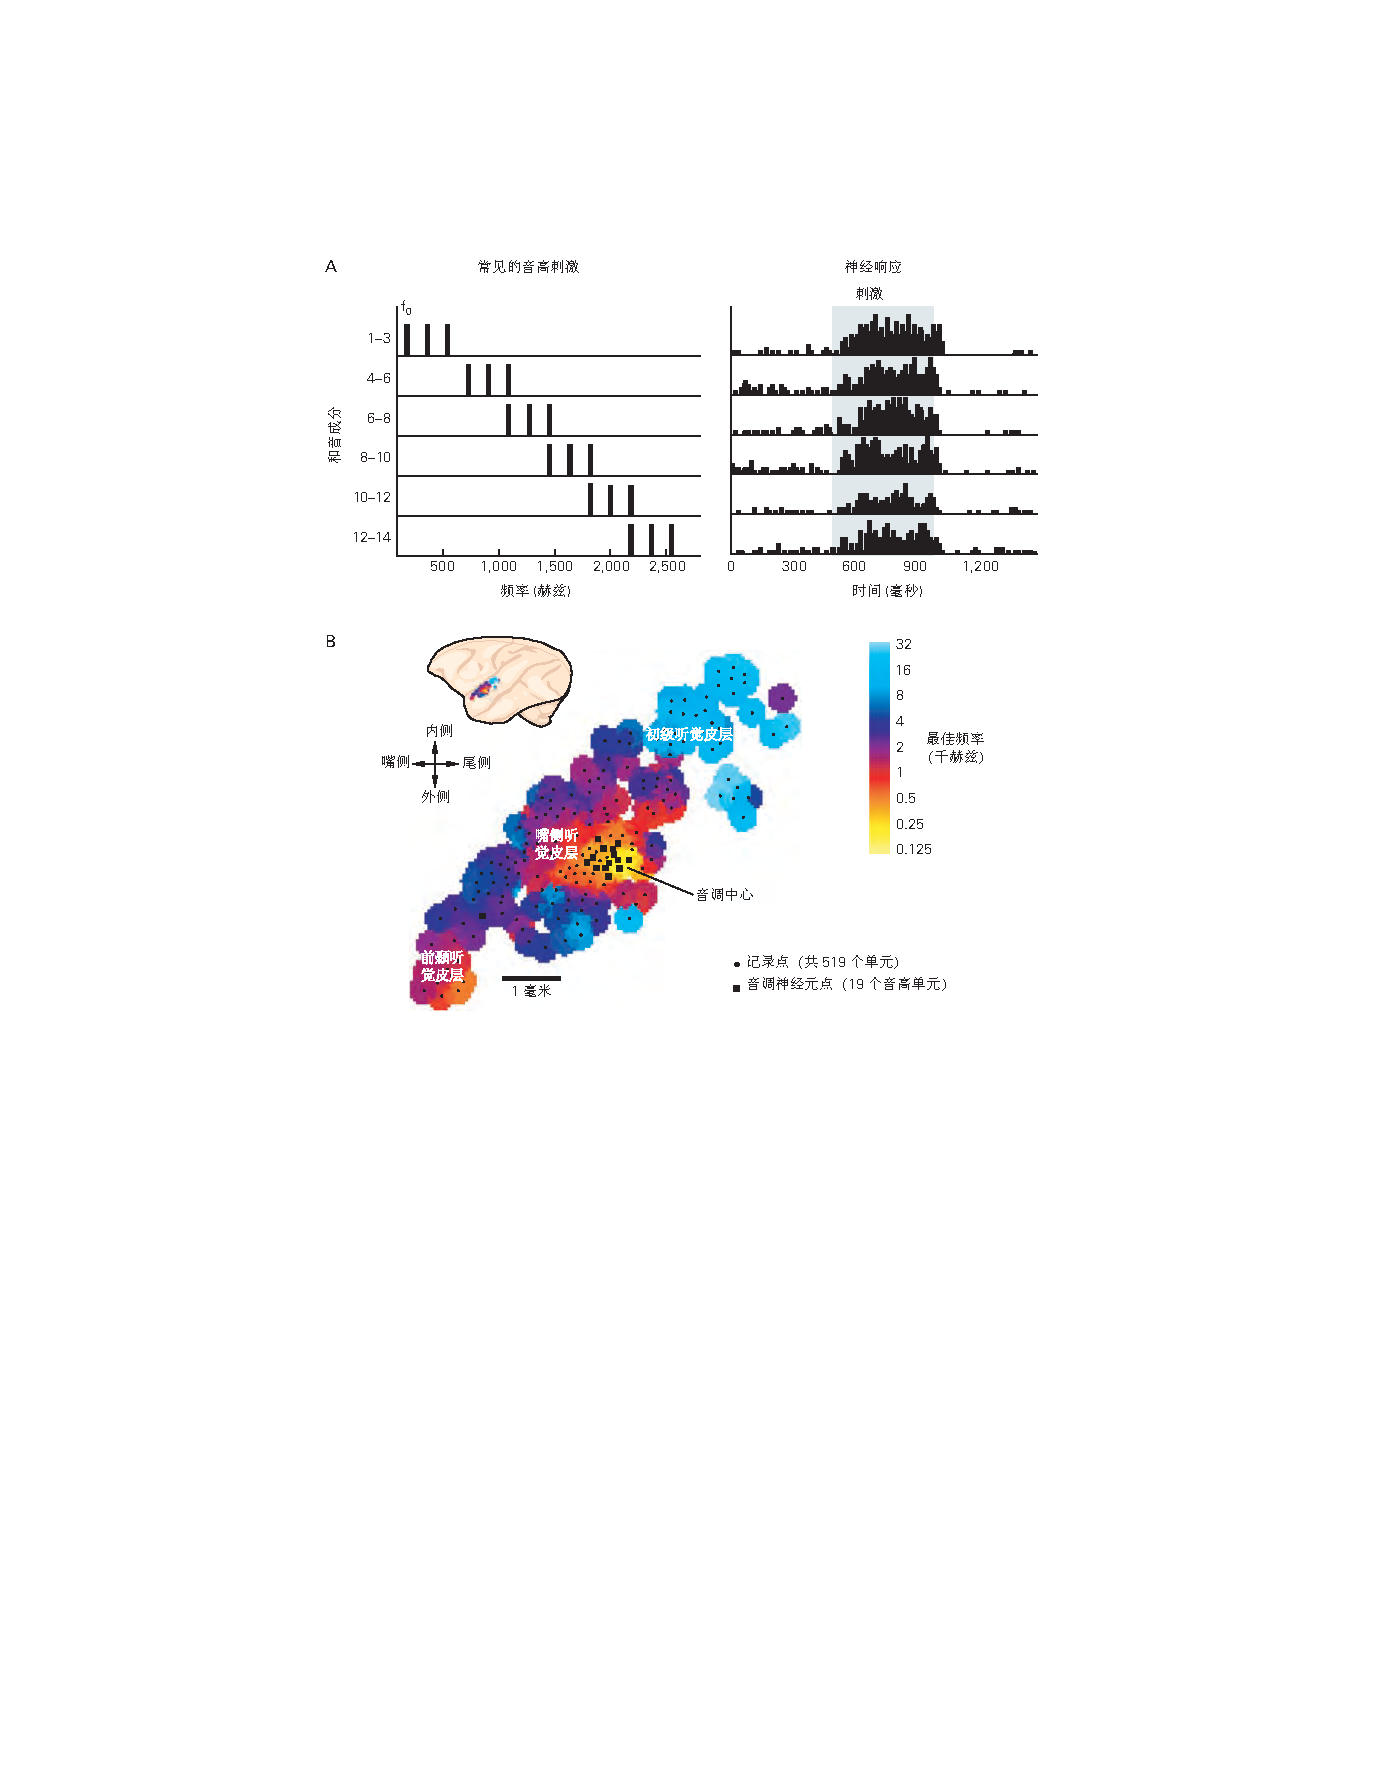
\includegraphics[width=0.85\linewidth]{chap28/fig_28_13}
	\caption{音调由灵长类动物听觉皮层中的专门神经元编码。
		A. 从狨猴听觉皮层记录的音高选择性神经元的例子。
		左图:一系列共享相同基频($f_0$)的谐波刺激频谱。
		右图:神经元对刺激响应的周围刺激时间直方图(阴影区域表示的刺激持续时间)\cite{bendor2005neuronal}。
		B. 狨猴听觉皮层的解剖组织和音高中心的位置。
		上图:狨猴大脑的侧视图。
		底部:一只狨猴典型的左听觉皮层音调图。
		音高选择性神经元(黑色方块)聚集在初级听觉皮层和嘴侧听觉皮层之间的低频边界附近。
		频率反转表示“初级听觉皮层/嘴侧听觉皮层”和“嘴侧听觉皮层/前颞听觉皮层”之间的边界\cite{bendor2005neuronal}。}
	\label{fig:28_13}
\end{figure}
% 周围刺激:与特定刺激事件相关的一段时间,通常用于神经科学和心理学研究中,以研究刺激前后的生理和行为响应。


当音调接近神经元的偏好最佳频率时,音调选择性神经元会对音高唤起声音(例如,和声、咔嗒声)做出响应。
随着音调的行为显著性增加,音调选择性神经元会增加它们的激活率,并且更喜欢周期性的声音而不是非周期性的声音。
重要的是要注意狨猴中的音调选择性神经元,它提取和编码嵌入谐波声音中的音调(高度非线性计算),明显不同于皮层下区域或仅“反映”音高信息的初级听觉皮层神经元在他们的激活模式中。


如图~\ref{fig:28_13}B~所示,狨猴中包含音调选择性神经元的区域仅限于初级听觉皮层的低频边界、嘴侧听觉皮层和外侧带状区。
人类成像研究已经确定了初级听觉皮层前外侧颞横回外侧端的一个有限区域,该区域提取谐波复杂声音的音高,并对音高显著性的变化敏感。
如图~\ref{fig:28_13}B~所示,该区域的位置反映了狨猴的音高中心位置。


狨猴听觉皮层的核心区域也包含一类谐波模板神经元,它们对纯音或双音组合响应微弱或根本不响应,但对多重谐波的特定组合响应强烈。
谐波模板神经元对谐波声音的响应比非谐波声音更强,并且对特定谐波结构具有选择性。
与位于初级听觉皮层和嘴侧听觉皮层之间低频边界外侧的小皮层区域内并且最佳频率小于 1 千赫兹的音调选择性神经元不同,谐波模板神经元分布在初级听觉皮层和嘴侧听觉皮层中,并且具有最佳频率范围从大约 1 千赫兹到大约 32 千赫兹,这个范围涵盖了狨猴的整个听觉范围。


% 谐波:电流中所含有的频率为基波的整数倍的电量
而在外围,单个听觉神经纤维编码谐波声音的各个分量,而谐波模板神经元的特性揭示了用于提取谐波模式的谐波结构感受野。
从听觉神经纤维到听觉皮层的和音神经表征变化反映了感觉系统中神经编码的原理。
感觉通路中的神经元将物理特征的表示(例如听觉中的声音频率或视觉中的图像亮度)转换为感知特征的表示,例如听觉中的音高或视觉中的曲率。
这些特征导致听觉认知或视觉认知的形成。
听觉皮层中的谐波模板神经元是处理具有谐波结构的声音的关键,例如动物发声、人类语言和音乐。



\subsection{食虫蝙蝠有皮层区域专门负责行为相关的声音特征}

虽然人们普遍认为上游听觉区执行与听觉相关的越来越特化的功能,但与视觉系统相比,人们对听觉系统中串行中继的功能知之甚少。
人类听觉最重要的作用之一就是处理语言,但我们对分析说话声音的神经回路知之甚少。
人类大脑成像的新技术逐渐提供了对与语言相关的皮层区域功能特化的见解(第~\ref{chap:chap55}~章)。


专门分析大脑皮层中复杂听觉信号的证据来自对食虫蝙蝠的研究。
这些动物几乎完全通过回声定位来找到猎物,发出的超声波脉冲被飞行昆虫反射。
蝙蝠分析回声的时间和结构来帮助定位并识别目标,而离散的听觉区域专门处理不同方向的回声。


许多蝙蝠,例如大胡子蝙蝠,都会发出具有 2 种成分的回声定位脉冲\cite{suga1983specificity,suga1984neural}。
初始\emph{恒频}分量由多个谐波相关的声音组成。 % \textit
这些谐波会稳定地发出几十到几百毫秒,类似于人类的元音。
如图~\ref{fig:28_14}A~所示,恒频分量之后是频率急剧下降的声音,\textit{调频}分量,类似于人类辅音的快速变化频率。


\begin{figure}[htbp]
	\centering
	\includegraphics[width=0.67\linewidth]{chap28/fig_28_14}
	\caption{蝙蝠的听觉系统有专门的区域来定位声音。
		A. 动物叫声声波图(实线)和由此产生的回声(虚线)说明了叫声的 2 个组成部分:延长的、谐波相关的恒频信号和较短的调频信号。
		当动物接近其目标时,呼叫的持续时间会缩短\cite{suga1984neural}。
		B. 大胡子蝙蝠的大脑半球视图显示了听觉皮层内的 3 个功能区域。
		调频区域是计算与目标的距离的地方;
		恒频区域是计算目标速度的地方;
		多普勒频移恒频区域专门用于识别小的颤动物体。
		在呼叫频率(60–62 千赫兹)的二次谐波附近,多普勒频移恒频信号的扩展皮层表示形成了声学“中央凹”\cite{suga1984neural}。
		C. 所示的"恒频-恒频"组合敏感神经元对单独的脉冲或回波没有显著响应,但对紧密配对的脉冲回波响应非常强烈。
		然而,神经元对脉冲和回波之间的时间差也很敏感,如右侧的记录所示,神经元无法响应未紧密配对的脉冲-回波组合\cite{suga1983specificity}。}
	\label{fig:28_14}
\end{figure}


调频声音用于确定到目标的距离。
蝙蝠根据相对恒定的声速测量发出的声音和返回的回声之间的间隔,该间隔对应于特定距离。
如图~\ref{fig:28_14}B~所示,听觉皮层“调频-调频” 区域的神经元优先响应由特定延迟分隔的脉冲回波对。
此外,这些神经元对特定声音组合的响应比对单独声音的响应更好。
如图~\ref{fig:28_14}C~所示,这样的神经元被称为特征检测器。
如图~\ref{fig:28_14}B~所示,“调频-调频”区域包含一系列此类检测器,偏好延迟系统范围为 0.4 至 18 毫秒,对应于 7 至 280 厘米的目标范围。
这些神经元按列组织,每个列都对刺激频率和延迟的特定组合有响应。
通过这种方式,蝙蝠就像其下丘中的仓鸮一样,能够表现出一种听觉特征,而这种特征不能直接由感觉受体表现出来。


蝙蝠叫声的恒频分量用于确定目标相对于蝙蝠的速度和目标的声学图像。
当回声定位蝙蝠飞向昆虫时,昆虫反射的声音在蝙蝠耳朵处被多普勒频移到更高的频率,因为蝙蝠正朝着目标返回的声波移动,导致这些声波在其耳朵处相对加速。
同样,一只后退的昆虫会在蝙蝠的耳朵处产生频率降低的反射。
如图~\ref{fig:28_14}B~所示,“恒频-恒频”区域中的神经元被急剧调谐到接近激活频率或其谐波的频率组合。
每个神经元对特定基频的脉冲与对应于脉冲的一次或二次谐波的回波的组合响应最好,多普勒频移到特定程度。
与“调频-调频”区域一样,神经元不会单独响应脉冲或回波,而是响应 2 个恒频信号的组合。


“恒频-恒频”神经元按列排列,每个列编码特定的频率组合。
这些列沿皮层表面规则排列,基频沿一个轴,回声谐波沿垂直轴。
这种双频坐标系创建了一个映射,其中特定位置对应于特定的多普勒频移,因此对应于特定的目标速度,范围从 –2 米/秒到 9 米/秒。


返回回波的恒频分量也用于声学图像的详细频率分析,可能在其识别中很重要。
如图~\ref{fig:28_14}B~所示,胡须蝙蝠的多普勒频移恒频区是初级听觉皮层对 60 千赫兹至 62 千赫兹频率表示的显著扩展,与蝙蝠叫声的主要恒频成分的一组返回回波非常对应。
在多普勒频移恒频区域内,单个神经元被极其敏锐地调谐到频率,因此很容易检测到飞蛾翅膀颤动所产生的微小频率变化。


当蝙蝠执行辨别任务时,这些专门的皮层区域中的一些暂时失活,这显著地支持了它们在行为中的功能专业化的重要性。
多普勒频移恒频的沉默有选择地削弱精细频率辨别,同时保持时间感知完好无损。
相反,“调频-调频”区域的失活会削弱蝙蝠检测 2 个回声到达时间的微小差异的能力,同时保持频率感知不变。


对与蝙蝠相关刺激的了解极大地促进了对这种听觉系统的研究。
这些皮层区域在功能上或解剖学上是否类似于猫、猴子和人类的特定区域还有待观察。
无论如何,选择合适的刺激物在研究这些其他物种时可能与在蝙蝠研究中一样重要。



\subsection{听觉皮层涉及处理说话时的声音反馈}

声音交流包括说话和听觉,通常同时发生。
当我们说话时,我们的声音不仅会传递给预期的听众,还会传回我们自己的耳朵。
在发声过程中,这种对我们听觉系统的反馈不仅通过空气进行,还通过骨骼进行,并且由于嘴和耳朵的接近而可能很响亮。


听觉系统必须区分听觉感知是自我产生的还是外部产生的。
为了在说话过程中监测来自声学环境的外部声音,必须屏蔽自身产生的声音。
同时,听觉系统还必须监测我们自己的声音,以检测发声中的错误。
通过声音反馈准确表达自己的声音对于保持理想的发声和学习新语言至关重要。
在人类和动物中,声音反馈的扰动会导致声音产生的改变,而声音反馈的中断或阻塞会导致声音学习的退化。
听觉皮层参与处理声音反馈的证据来自人类和动物研究。
说话时人类受试者的听觉皮层对自己声音的响应小于对相同声音回放的响应。
如图~\ref{fig:28_15}A~所示,这种减少可以在脑电图记录或各种成像方法(例如,功能性核磁共振成像、正电子发射断层成像、脑磁图)中观察到。


\begin{figure}[htbp]
	\centering
	\includegraphics[width=1.0\linewidth]{chap28/fig_28_15}
	\caption{听觉皮层的声音反馈处理。
		A. 发声引起的抑制和对人类大脑皮层音调扰动的敏感性的例子。
	1. 受试者的发声(红色箭头)通过数字信号处理器,该处理器改变音调并将失真的听觉反馈(蓝色箭头)传送到受试者的耳机。 
	2. 示例试验的音调轨迹显示了麦克风记录的音调(产生)和传送到耳机的音调(听到)。
	阴影区域表示信号处理器将音高移动 −200 音分(1 音分 = 1/1200 倍频程)时的时间间隔。
	3. 从颞上回表面听觉皮层的 2 个位置记录的电极位置。
	4. Z 变量表示皮层活动在 50 至 150 赫兹(高 $\gamma$)范围内的功率,这已被证明与神经元脉冲活动密切相关。 
	它是从每个电极在说话(红色)和听力(蓝色)条件下记录的信号中提取的。
	图左栏中的垂直线表示发声开始,图右栏中的阴影区域表示扰动的开始和偏移。
	受试者的听觉皮层对其自己发声的响应通常小于受试者被动聆听相同发声回放时的响应(左栏)。 
	听觉皮层在主动发声(说话)期间对扰动的响应得到增强(右栏)\cite{houde2015cortical}。
	B. 1. 发声诱导的狨猴听觉皮层神经活动抑制。 
	所有发声抑制响应的群体平均激活率与发声(“Phee”呼叫)一致。 
	蓝线是移动平均值(100 毫秒窗口),表明抑制在发声之前开始(用箭头表示)。 
	粗条表示抑制持续显著的时期(P<0.05)\cite{eliades2003sensory}。
	2. 受到发声诱导抑制的神经元对声音反馈扰动很敏感。
	上图:通过定制的耳机将带或不带反馈改变的自制发声传送到狨猴。
	底部:这个听觉皮层神经元在正常发声(深蓝色)期间被抑制,但当发声的听觉反馈在频域(浅蓝色)中移动时,其激活率显著增加。
	单独放大听觉反馈不会产生激活率变化(黑色)\cite{eliades2008neural}。}
	\label{fig:28_15}
\end{figure}


如图~\ref{fig:28_15}B~所示,来自发声猴听觉皮层的单神经元记录表明,自发发声导致皮层对猴子自身发声的响应、发声期间听到的外部声音以及自发活动的抑制。
因为在许多情况下,激活率被抑制到低于自发活动,抑制很可能是由抑制引起的。
被自发发声抑制的神经元表现出频率和强度调谐,这是听觉皮层神经元的典型特征,并对发声的回放做出响应。


如图~\ref{fig:28_15}B~所示,发声诱导的抑制在发声开始前几百毫秒开始,表明这些神经元接收来自发声回路的调制信号。
在人类中,声音的产生是由额叶的皮层区域进行的,从布洛卡区到前运动和运动皮层。
在人类和猴子中,已经描述了从\textit{前运动皮层}到颞上回听觉区的轴突,并且据推测,它们介导了发声诱导的抑制。
当人类或猴子只是聆听播放给它们的声音时,这种调节连接并不活跃。


为什么我们说话时会抑制听觉皮层?
一个简单的答案是,这种抑制有助于降低我们自己声音的遮蔽效果,这种声音可能非常响亮。
一个更有趣的答案是,这种抑制是由听觉皮层中的声音反馈监控网络引起的。
如图~\ref{fig:28_15}A~所示,在人类中,如果通过耳机实验性地改变声音反馈,例如,当声音的音高发生变化时,听觉皮层的抑制就会减少或没有。
如图~\ref{fig:28_15}C~所示,在狨猴中,当动物听到自己的频移发声时,被自发发声抑制的神经元可能变得不那么抑制甚至兴奋。
这种对反馈扰动的敏感性表明,表现出发声诱导抑制的神经元是负责监测声音反馈信号的网络的一部分。
人类和猴子听觉皮层中声音反馈相关神经活动的存在表明听觉皮层结合了内部调制和声音反馈响应,而不仅仅是对通过耳朵传来的感觉信号做出响应。


并非听觉皮层中的所有神经元都会因说话或发声而受到抑制。
狨猴初级听觉皮层中较小比例(30\%)的神经元在自发发声期间增加了它们的响应,这与其听觉响应特征一致。
与发声诱导的抑制相反,发声相关的兴奋在发声开始后开始,并且可能是通过上行听觉通路反馈的结果。
与发声相关的兴奋可能有助于在说话或发声期间保持听觉皮层对外部声学环境的敏感性。


已经在几种哺乳动物皮层下结构(包括脑干和下丘)中观察到发声诱导的听觉响应抑制。
这种抑制在声音产生前几毫秒开始或与声音产生同步。
相比之下,皮层抑制在发声前几百毫秒就开始了。
说话或发声期间听觉响应的皮层下抑制可能是由皮层指令启动的。



\section{要点}

1. 撞击在两只耳朵上的声音携带着大脑用来计算声音出现的位置及其含义的信息。
声音的特征在于一个或多个频率的能量大小。
为了确定声音在水平面的何处出现,许多哺乳动物计算小于大约 3 千赫兹的声音到达两只耳朵的时间差异。
为了确定声音在垂直方向上出现的位置以及它们是从前面还是后面发出,哺乳动物使用头部、肩部和外耳对大于大约 6 千赫兹的声音进行频谱过滤。 


2. 听觉神经纤维将声音信息从耳蜗传送到大脑,每条神经纤维都被急剧调谐到一个狭窄的频率范围,并共同代表动物的整个听觉范围。
听觉神经纤维终止于腹侧耳蜗核和背侧耳蜗核,将声学信息分配给 4 个主要的主要细胞群,形成通过脑干的并行上行通路。
听觉神经输入的拓扑组织赋予同侧耳蜗核一个音调组织,该组织在整个听觉通路(包括听觉皮层)中得到保留。


3. 沿着上行通路的处理站处的听觉神经元的一个显著特征是它们逐渐增加的刺激选择性。


4. 腹侧耳蜗核提取声音的 3 个特征:
(a)通过腹侧耳蜗核、上橄榄核和外侧丘系腹侧核的章鱼细胞的单耳通路检测听觉神经纤维的同步激活,这有助于 检测声音的开始和间隙。
(b)星状细胞检测并锐化光谱峰谷的编码,并将光谱信息传递给背侧耳蜗核、外侧丘系腹核、外侧丘系腹侧核、下丘和丘脑中的橄榄耳蜗神经元。 
频谱信息用于理解声音的含义和定位其来源。 
(c)丛细胞锐化并传递有关声音精细结构的信息,这些信息用于通过内侧和外侧上橄榄核的双耳通路,以对两只耳朵的声音时间和强度进行耳间比较,用于沿方位定位声源。


5. 耳蜗背侧核在其主要细胞中整合声学信号和体感信息。
体感信息有助于将动物自身运动产生的光谱线索与环境产生的光谱线索区分开来,这些线索在生物学上是无趣的。


6. 听觉脑干通路汇聚于下丘。
下丘通过丘脑的内侧膝状体向听觉皮层提供声学信息

 

7. 来自下丘的投射将关于声音位置的信息传送到上丘,上丘是控制头部和眼睛的反射性定向运动的大脑的一部分。 

8. 在听觉皮层内,听觉神经元继续变得对它们响应的刺激更具选择性。
听觉皮层的子区域代表不同的生物学重要特征,例如形成谐波复合体的音高。
听觉皮层还将快速变化的声音特征转换为基于激活率的表示,同时使用脉冲时间表示缓慢变化的声音。


9. 大脑皮层中的听觉回路被分成不同的处理流,背侧和腹侧流分别与声音在空间中的定位和声音识别有关。 

10. 大脑皮层调节皮层下听觉区的处理。
来自听觉皮层的投射支配丘脑、下丘、橄榄耳蜗神经元、一些基底神经节结构,甚至耳蜗背核。


11. 听觉皮层参与处理说话时的声音反馈信号。
说话会抑制听觉皮层的神经活动,这种活动在发声前几百毫秒就开始了。
这种抑制是声音反馈监测网络的结果,该网络的作用是指导声音的产生和学习。

